\section{Image Processing}
\label{sec: imageProcessing}
\tododone[inline]{Saumi}{\textbf{Image Processing} done.}
\tododone[inline]{Benni}{Someone proofreading?: Proofreading done: Saumi}

One of Grand Theft Boat's USPs is the freedom for players to fully customize their level maps. Players can design complex maps replete with shorelines, connected water bodies, and floating spherical obstacles of varying radii. All this can be done using a simple computer graphics software like Gimp (Linux), MS Paint (Windows) and Paintbrush (Mac). 

\begin{figure}
\centering
  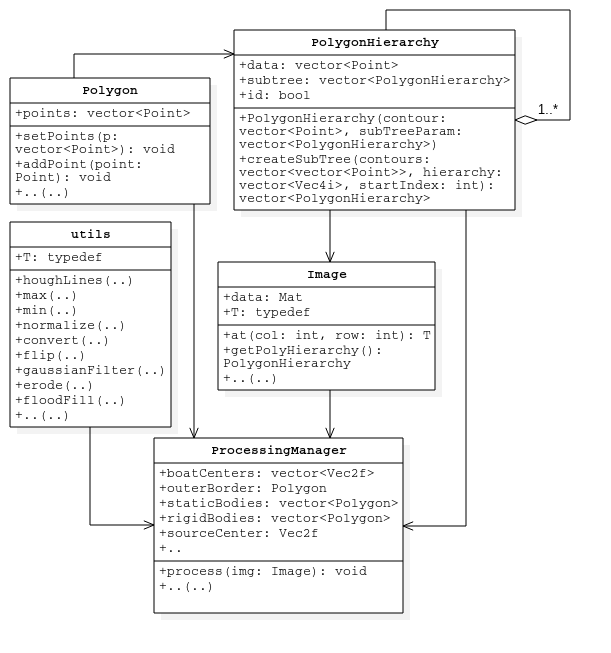
\includegraphics[scale=0.6]{img/ImageProcessing/UML_ImgProc_PNG.png}
\caption{UML diagram for the image processing code\label{fig:UMLImgProc}}
\end{figure}

In order to extract information about the terrain and participating bodies, the team relied on processing the input image through extensive use of the OpenCV library. This chapter describes the workflow involved in this stage. The broad structure of the image processing code is shown in Figure \ref{fig:UMLImgProc}.

The other parts of the code interact with the Image Processing section through an instance of \verb|ProcessingManager|. This class takes an image from the player, processes it to extract and store information about different terrain objects, and provides functions to return this information when required by other sections.

\subsection{Level Terrain Specification}

\begin{figure}
\centering
  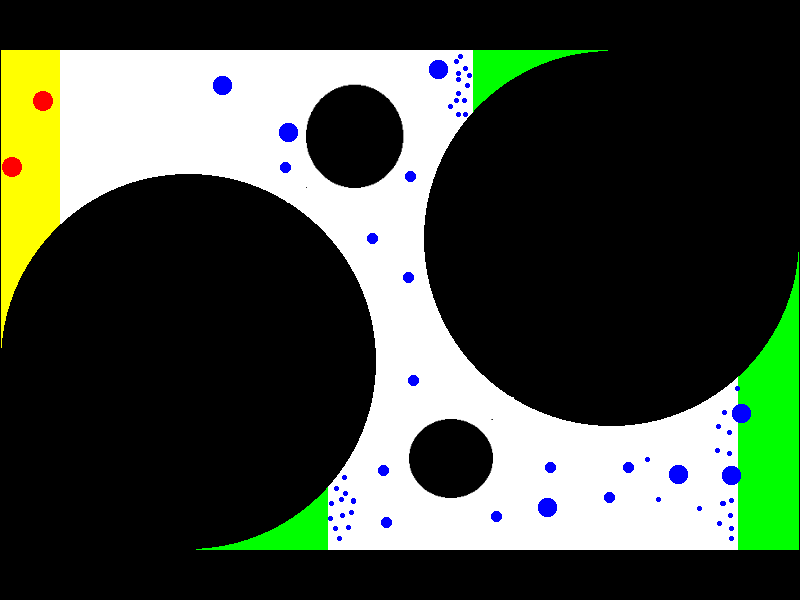
\includegraphics[scale=0.4]{img/ImageProcessing/LevelImages/img_0.png}
\caption{A typical player input for specifying the desired layout of the level\label{fig:LevelInput}}
\end{figure}

Figure \ref{fig:LevelInput} shows an example of a player's level specification.
\begin{itemize}
	\item Regions colored black represent land. This part of the domain is not a part of the solution field. The part of the black that borders the white region is treated as a rigid boundary.
	\item White-colored regions represent the water body. This space is the actual solution domain of the fluid.
	\item Green patches represent sources of momentum for the fluid.
	\item Yellow patches are sinks for the fluid. (See the section on LBM for the mathematical meaning of sources and sinks.
	\item Red spheres indicate the initial position of the player boats.
	\item Blue spheres create obstacles as rigid bodies.
\end{itemize}


\subsection{Pre-Processing}

Many a time, the image supplied by the player may need to be pre-processed for improving boundaries between terrain types. Once given as input to the \verb|ProcessingManager|, the input image undergoes the following sequence of filters:

\begin{enumerate}
	\item \textit{Flip image}: 
	
	\verb|img = img::flip(img, true, false);|
	
	Flipping the image along the y-axis is necessary because the coordinate system of a standard image has its origin on the top-left corner, while standard fluid codes begin indexing from the bottom-left corner.

	\item \textit{Gaussian filter and opening}

	\verb|blurred = img::gaussianFilter(img, 7, 2);|

	\verb|opened = img::opening(blurred, structuringElement, 2);|
	
	The gaussian filter and opening helps eliminates fuzzy borders of adjacent colors, making them sharper. See Figure \ref{LevelImages}(a).

	\item \textit{Thresholding}

	\verb|thresholded = applyThresholding(opened);|
	
	Thresholding applies yes-no filters on the image based on the colors of different domain types. This provides the \verb|ProcessingManager| with a boolean (black-white) image for each domain type, which is then used to extract domain information.

\end{enumerate}


\subsection{Information Extraction}

\begin{figure}
\begin{tabular}{cc}
  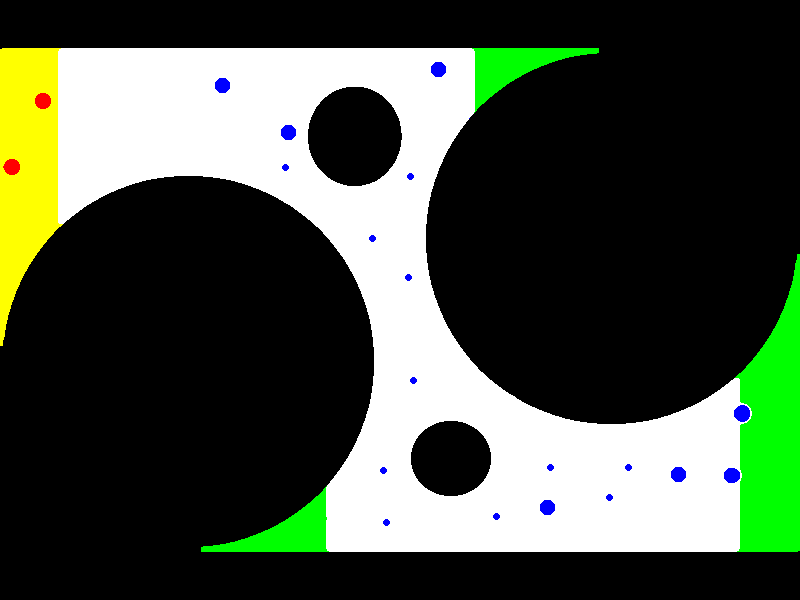
\includegraphics[width=65mm]{img/ImageProcessing/LevelImages/img_3.png} & 
\includegraphics[width=65mm]{img/ImageProcessing/LevelImages/img_5.png} \\
(a) & (b) \\[6pt]
  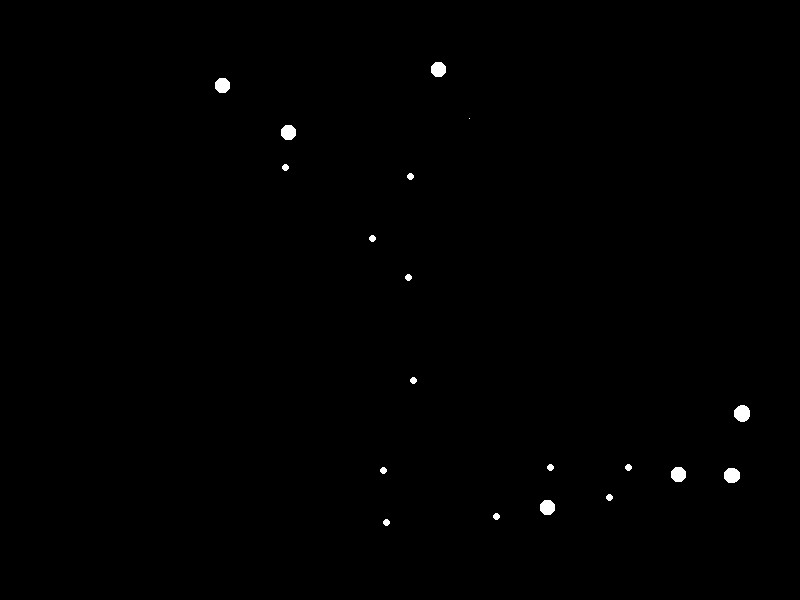
\includegraphics[width=65mm]{img/ImageProcessing/LevelImages/img_10.png} & 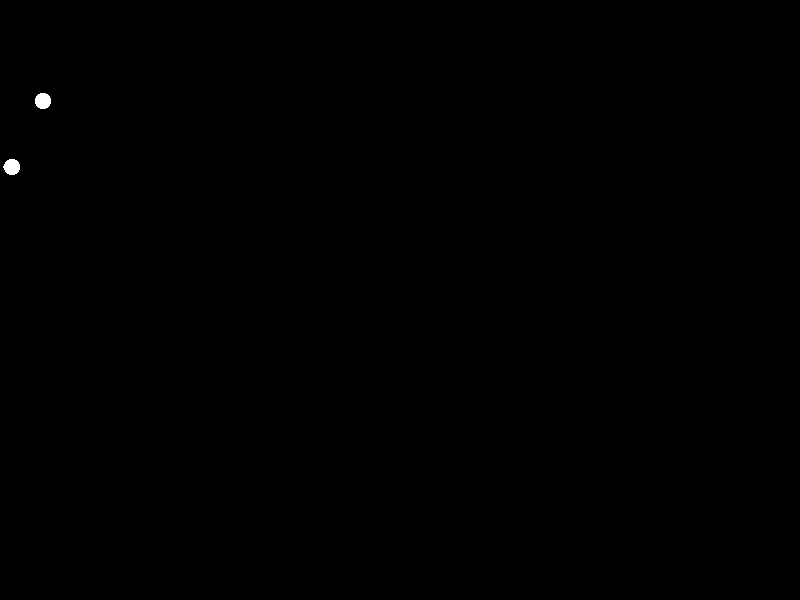
\includegraphics[width=65mm]{img/ImageProcessing/LevelImages/img_12.png} \\
(c) & (d) \\[6pt]
\end{tabular}
\caption{Various stages of processing the image. (a) After pre-processing, (b) image for \protect\lstinline|outerBorder| and \protect\lstinline|staticBodies|, (c) image for \protect\lstinline|rigidBodies|, and (d) image for \protect\lstinline|boatCenters|.\label{LevelImages}}
\end{figure}

The pre-processing brings the image in a state where information about the terrain can be easily extracted from it. Various information extraction techniques are applied to this processed image to obtain terrain information relevant to the simulation.

\begin{itemize}
	\item \textit{Sources}: Detected by a simple color comparison.
	\item \textit{Boats}: Boat pixels detected by color comparison. Their centers are located by a k-means analysis for 2 buckets. See Figure \ref{LevelImages}(d)
	\item \textit{Rigid Bodies}: The first step in the detection of the rigid body obstacles is the isolation of the obstacles as a binary "obstacle or not-obstacle" image. This is done by a series of boolean operations (provided in class \lstinline|utils|). This image is then supplied to the class \lstinline|PolygonHierarchy|.

The class \lstinline|PolygonHierarchy| is a recursive class holding two parameters: 
	\begin{itemize}
		\item \lstinline|data|: a set of points forming a closed polygon.
		\item \lstinline|subtree|: a vector of \lstinline|PolygonHierarchy|.
	\end{itemize}
The level of a \lstinline|PolygonHierarchy| indicates how many outer polygons enclose the polygons at that level. Note that the zeroeth-level \lstinline|data| is empty.

This \lstinline|PolygonHierarchy| is applied on Figure \ref{LevelImages}(c), and the first-level polygons give the rigid body obstacles.

	\item \textit{Fluid Domain}: The fluid domain is extracted in a similar manner by choosing the first-level polygon for Figure \ref{LevelImages}(b).

	\item \textit{Static Bodies}: The static bodies are detected by choosing the second-level polygons for Figure \ref{LevelImages}(b).

\end{itemize}


The Image-processing-group also performs the task of writing the flag field for the LBM-group. The flag field is scaled to the desired screen pixel resolution. All the information extracted so far is stored in the \verb|ProcessingManager| and passed on to the Rigid-body-group (for obstacles, shorelines and boats) and the LBM-group (for the flag fields).
